\documentclass[a4paper,12pt,titlepage,finall]{article}

\usepackage[T1,T2A]{fontenc}     % форматы шрифтов
\usepackage[utf8x]{inputenc}     % кодировка символов, используемая в данном файле
\usepackage[russian]{babel}      % пакет русификации
\usepackage{tikz}                % для создания иллюстраций
\usepackage{pgfplots}            % для вывода графиков функций
\usepackage{geometry}		 % для настройки размера полей
\usepackage{indentfirst}         % для отступа в первом абзаце секции

% выбираем размер листа А4, все поля ставим по 3см
\geometry{a4paper,left=30mm,top=30mm,bottom=30mm,right=30mm}

\setcounter{secnumdepth}{0}      % отключаем нумерацию секций

\usepgfplotslibrary{fillbetween} % для изображения областей на графиках

\pgfplotsset{compat=1.15}
\begin{document}
% Титульный лист
\begin{titlepage}
    \begin{center}
	{\small \sc Московский государственный университет \\имени М.~В.~Ломоносова\\
	Факультет вычислительной математики и кибернетики\\}
	\vfill
	{\Large \sc Отчет по заданию №6}\\
	~\\
	{\large \bf <<Сборка многомодульных программ. \\
	Вычисление корней уравнений и определенных интегралов.>>}\\ 
	~\\
	{\large \bf Вариант 2 / 2 / 2}
    \end{center}
    \begin{flushright}
	\vfill {Выполнил:\\
	студент 103 группы\\
	Иванов~М.~Ю.\\
	~\\
	Преподаватель:\\
	Кузьменкова~Е.~А.}
    \end{flushright}
    \begin{center}
	\vfill
	{\small Москва\\2019}
    \end{center}
\end{titlepage}

% Автоматически генерируем оглавление на отдельной странице
\tableofcontents
\newpage

\section{Постановка задачи}

Необходимо реализовать многомодульную программу, вычисляющую площадь плоской фигуры, ограниченной графиками трех функций с заданной точностью $\varepsilon$. Для нахождения вершин фигуры использовался \textbf{метод хорд}. Отрезок для применения данного метода должен быть вычислен аналитически. Подсчет площади плоской фигуры производился с помощью \textbf{метода трапеций}.

\section{Математическое обоснование}

\subsection{Функции}

Необходимо было найти площадь между тремя кривыми, заданных функциями:

\begin{enumerate}
    \item $f_1=3*(\frac{0.5}{(x+1)}+1)$
    \item $f_2=2.5*x-9.5$
    \item $f_3=\frac{5}{x}$
\end{enumerate}

Ниже приведены графики данных функций (рис.~\ref{plot1}).

\begin{figure}[h]
\centering
\begin{tikzpicture}
\begin{axis}[grid=both,                % рисуем координатную сетку (если нужно)
             axis lines=middle,          % рисуем оси координат в привычном для математики месте
             restrict x to domain=-1:7,  % задаем диапазон значений переменной x
             restrict y to domain=-1:7,  % задаем диапазон значений функции y(x)
             axis equal,                 % требуем соблюдения пропорций по осям x и y
             enlargelimits,              % разрешаем при необходимости увеличивать диапазоны переменных
             legend cell align=left,     % задаем выравнивание в рамке обозначений
             scale=2]                    % задаем масштаб 2:1

% первая функция
% параметр samples отвечает за качество прорисовки
\addplot[green,domain=-1:7,samples=256,thick] {3*(0.5/(x+1)+1)};
% описание первой функции
\addlegendentry{$y=3*(\frac{0.5}{(x+1)}+1)$}

% добавим немного пустого места между описанием первой и второй функций
\addlegendimage{empty legend}\addlegendentry{}

% вторая функция
% здесь необходимо дополнительно ограничить диапазон значений переменной x
\addplot[blue,domain=-1:7,samples=256,thick] {2.5*x-9.5};
\addlegendentry{$y=2.5*x-9.5$}

% дополнительное пустое место не требуется, так как формулы имеют небольшой размер по высоте

% третья функция
\addplot[red,domain=-1:7,samples=256,thick] {5/x};
\addlegendentry{$y=\frac{5}{x}$}
\end{axis}
\end{tikzpicture}
\caption{Плоская фигура, ограниченная графиками заданных уравнений}
\label{plot1}
\end{figure}

\subsection{Поиск корней}

Нахождение корней проводилось с помощью \textbf{метода хорд} с вычислительной точностью $\varepsilon_1=0.001$ на промежутке $[0.5, 7]$.
Для использования данного метода необходимо выполнение следующих условий на отрезке $[a, b]$:

\begin{enumerate}
    \item $F(x)\in C^1[a, b]$;
    \item $F(a)*F(b) < 0$;
    \item $F'(x)$ монотонна на $[a, b]$;
    \item $F'(x)$ сохраняет знак на $[a, b]$.~x\cite{math}
\end{enumerate}

\subsection{Поиск интеграла}

Интегрирование проводилось \textbf{методом трапеций} с вычислительной точностью $\varepsilon_2=0.001$.

\newpage

\subsection{Обоснавание выбора промежутка $[a, b]$}

Ниже приведено математическое обоснование выполнения условий применимости \textbf{метода хорд} поиска корней на промежутке $[0.5, 7]$.

\begin{enumerate}

    \item $F_{12}(x) = 3*(\frac{0.5}{(x+1)}+1) - 2.5*x + 9.5$
    \begin{enumerate}
        \item $F'_{12}(x) = -\frac{3}{2(x+1)^2}-2.5$
        \\*Производная функции непрерывна на промежутке $[0.5, 7]$.
        \item $F_{12}(0.5) = 4 + 8.25 = 12.25 > 0$,
        \\*$F_{12}(7) = \frac{51}{16} + 8 = -\frac{77}{17} < 0$
        \\*Тогда $F_{12}(0.5) * F_{12}(7) < 0$.
        \item $F''_{12}(x) = \frac{3}{(x+1)^3} > 0$ (на промежутке $[0.5, 7]) =>$ первая производная возрастает на этом промежутке.
        \item $F'_{12}(x) < 0$ на всем промежутке $[0.5, 7]$.
    \end{enumerate}
    
    \item $F_{13}(x) = 3*(\frac{0.5}{(x+1)}+1) - \frac{5}{x}$
    \begin{enumerate}
        \item $F'_{13}(x) = -\frac{3}{2(x+1)^2} + \frac{5}{x^2}$
        \\*Производная функции непрерывна на промежутке $[0.5, 7]$.
        \item $F_{13}(0.5) = 4 - 10 = -6 < 0$,
        \\* $F_{13}(7) = \frac{51}{16} - \frac{5}{7} > 0$
        \\*Тогда $F_{13}(0.5) * F_{13}(7) < 0$.
        \item $F''_{13}(x) = \frac{3}{(x+1)^3} - \frac{10}{x^3}$
        \\* $F'''_{13}(x) = 3*(-\frac{3}{(x+1)^4} + \frac{10}{x^4}) = 0$ только при $x < 0$, значит $F''_{13}(x)$ возрастает на промежутке $[a, b]$, так как  $F'''_{13}(1) = 3*(-\frac{3}{16} + 10) > 0$.
        \\* При этом $F''_{13}(7) = \frac{3}{8^3} - \frac{10}{7^3} = \frac{3*7^3 - 10*8^3}{56^3} < 0 =>$ $F''_{13}(x) < 0$ на всем промежутке $[a, b]$, тогда  $F'_{13}(x)$ убывает на данном промежутке.
        \item $F'_{13}(7) = -\frac{3}{128} + \frac{5}{49} > 0$, тогда так как $F'_{13}(x)$ убывает на всем промежутке $[0.5, 7]$, то  $F'_{12}(x) > 0$ на данном промежутке.
    \end{enumerate}
    
    \item $F_{23}(x) = 2.5*x - 9.5 - \frac{5}{x}$
    \begin{enumerate}
        \item $F'_{23}(x) = 2.5 + \frac{5}{x^2}$
        \\*Производная функции непрерывна на промежутке $[0.5, 7]$.
        \item $F_{23}(0.5) = -8.25 - 10 < 0$,
        \\*$F_{23}(7) = 8 - \frac{5}{8} > 0$
        \\*Тогда $F_{23}(0.5) * F_{23}(7) < 0$.
        \item $F''_{23}(x) = -\frac{10}{x^3} < 0$ (на промежутке $[0.5, 7]) =>$ первая производная убывает на этом промежутке.
        \item $F'_{23}(x) > 0$ на всем промежутке $[0.5, 7]$.
    \end{enumerate}
    
\end{enumerate}

\subsection{Значения $\varepsilon_1$ и $\varepsilon_2$}

При вычислении корней методом хорд имеется погрешность, которая вычисляется по формуле $|x_n-x_{n-1}|<\frac{|F(x_n)|}{m}=\varepsilon_1$, где $m$ - минимальное значение модуля первой производной на сегменте $[a, b]$.~\cite{math}

При вычислении площадей методом трапеции имеется погрешность $R=-\frac{F''(\xi)}{12n^2}(b-a)^3=\varepsilon_2$, где $a\leq\xi\leq b$, $n$ - число разбиений отрезка $[a, b]$ на равные части, $a, b$ - корни уравнений.~\cite{math}

\newpage

\section{Результаты экспериментов}

Координаты точек пересечения представлены в таблице (таблица~\ref{table1}) и на графике (рис.~\ref{plot2}). 
\textbf{Площадь фигуры, заключенной между кривыми, равна $S = 5.087$} (рис.~\ref{plot2}).

\begin{table}[h]
\centering
\begin{tabular}{|c|c|c|}
\hline
Кривые & $x$ & $y$ \\
\hline
1 и 2 & 5.078 & 3.247 \\
2 и 3 & 1.375 & 3.632 \\
1 и 3 & 4.267 & 1.168 \\
\hline
\end{tabular}
\caption{Координаты точек пересечения}
\label{table1}
\end{table}

\begin{figure}[h]
\centering
\begin{tikzpicture}
\begin{axis}[% grid=both,                % рисуем координатную сетку (если нужно)
             axis lines=middle,          % рисуем оси координат в привычном для математики месте
             restrict x to domain=-1:7,  % задаем диапазон значений переменной x
             restrict y to domain=-1:7,  % задаем диапазон значений функции y(x)
             axis equal,                 % требуем соблюдения пропорций по осям x и y
             enlargelimits,              % разрешаем при необходимости увеличивать диапазоны переменных
             legend cell align=left,     % задаем выравнивание в рамке обозначений
             scale=2,                    % задаем масштаб 2:1
             xticklabels={,,},           % убираем нумерацию с оси x
             yticklabels={,,}]           % убираем нумерацию с оси y

% первая функция
% параметр samples отвечает за качество прорисовки
\addplot[green,domain=-1:7,samples=256,thick, name path=A] {3*(0.5/(x+1)+1)};
% описание первой функции
\addlegendentry{$y=3*(\frac{0.5}{(x+1)}+1)$}

% добавим немного пустого места между описанием первой и второй функций
\addlegendimage{empty legend}\addlegendentry{}

% вторая функция
% здесь необходимо дополнительно ограничить диапазон значений переменной x
\addplot[blue,domain=-1:7,samples=256,thick, name path=B] {2.5*x-9.5};
\addlegendentry{$y=2.5*x-9.5$}

% дополнительное пустое место не требуется, так как формулы имеют небольшой размер по высоте

% третья функция
\addplot[red,domain=-1:7,samples=256,thick, name path=C] {5/x};
\addlegendentry{$y=\frac{5}{x}$}

% закрашиваем фигуру
\addplot[blue!20,samples=256] fill between[of=A and C,soft clip={domain=1.375:4.267}];
\addplot[blue!20,samples=256] fill between[of=A and B,soft clip={domain=4.263:5.078}];
\addlegendentry{$S=5.087$}

% Поскольку автоматическое вычисление точек пересечения кривых в TiKZ реализовать сложно,
% будем явно задавать координаты.
\addplot[dashed] coordinates { (5.078, 3.247) (5.078, 0) };
\addplot[color=black] coordinates {(5.078, 0)} node [label={-90:{\small 5.078}}]{};

\addplot[dashed] coordinates { (1.375, 3.632) (1.375, 0) };
\addplot[color=black] coordinates {(1.375, 0)} node [label={-90:{\small 1.375}}]{};

\addplot[dashed] coordinates { (4.267, 1.168) (4.267, 0) };
\addplot[color=black] coordinates {(4.267, 0)} node [label={-90:{\small 4.267}}]{};

\end{axis}
\end{tikzpicture}
\caption{Плоская фигура, ограниченная графиками заданных уравнений}
\label{plot2}
\end{figure}

\newpage

\section{Структура программы и спецификация функций}

\subsection{Вычислительный модуль}
В вычислительном модуле \textbf{calc.c} описаны следующие функции:

\begin{enumerate}
    \item double min(double a, double b)
    \\* Возвращает минимальное из чисел a и b
    \item double max(double a, double b)
    \\* Возвращает максимальное из чисел a и b
    \item int search\_max(double *x, int n)
    \\* Возвращает индекс максимального элемента в массиве вещесвенных чисел из n элементов
    \item int search\_mid3(double x[])
    \\* Возвращает средний элемент массива из 3 чисел по возрастанию
    \item double search\_delta(double (*f)(double), double x1, double x2, double eps)
    \\* Возвращает минимальное значение функции f, меньшее 0, или 0 на промежутке от x1 до x2.
    \item double integral(double (*f)(double), double a, double b, double eps, double delta)
    \\* Возвращает определенный интеграл функции f на промежутке от a до b с поднятием функции на delta.
    \item double root(double (*f)(double), double (*g)(double), double a, double b, double eps)
    \\* Возвращает координату абцисс точки пересечения функций f и g на отрезке от a до b.
\end{enumerate}

\subsection{Модуль функций}

В модуле \textbf{func.asm} описаны 3 функции основного задания, на вход каждой из которых подается вещественное число, а на выход - значение функции в заданной точке.

\subsection{Главный модуль}

В главном модуле \textbf{main.c} описаны следующие функции:

\begin{enumerate}
    \item int s\_in\_a(char *s, char *arr[], int n)
    \\* Проверяет наличие строки s в массиве строк arr размером n и возвращает индекс строки в массиве если она там есть и 0 иначе.
    \item double test\_f1(double x)
    \\* Тестовая функция 1. Возвращает значение функции в точке x.
    \item double test\_f2(double x)
    \\* Тестовая функция 2. Возвращает значение функции в точке x.
    \item double test\_f3(double x)
    \\* Тестовая функция 3. Возвращает значение функции в точке x.
    \item int main(int argc, char *argv[])
    \\* Главная функция модуля. В нем происходит подсчет площади и вывод ее на экран.
\end{enumerate}

\subsection{Библиотеки}

Помимо стандартных библиотек языка C, в программе задействована вспомогательная библиотека lib.h, в которую занесены все функции вспомогательных модулей.

\begin{figure}[h]
\center{\includegraphics[scale=0.5]{pic/diag.png}}
\caption{Схема использования функций и модулей друг другом.}
\label{fig:image}
\end{figure}

%\usepackage{graphicx}
%\graphicspath{{pictures/}}
%\DeclareGraphicsExtensions{.png}
%\includegraphics[width=\textwidth]{diag}

\newpage

\section{Сборка программы (Make-файл)}
Итоговый проект square.e собирается из 3 объектных модулей: \\ 
main.o func.o calc.o \\
Они в свою очередь собираются из 3 файлов: \\
main.c calc.c func.asm \\
Все фунцкии, использующиеся в программе, описаны в библиотеке: lib.h \\
Также используется библиотека: io.inc

Все модули находятся в папке \textsc{SRC}.

Итоговый проект состоит из следующих модулей:
\begin{itemize}
    \item main.c
    \\* Главный модуль. В нем происходит обработка опций, вводимых в командной строке. Также в нем происходит подсчет искомой площади фигуры.
    \item calc.c
    \\* Вычислительный модуль. В нем находятся функция, вычисляющая корни уравнений, функция, вычисляющая определенный интеграл и другие вспомогательные функции.
    \item func.asm
    \\* Модуль функций. В нем вычисляются функции, заданные условием задачи.
    \item lib.h
    \\* Библиотека. Здесь описаны прототипы всех используемых функций.
\end{itemize}

Для сборки проекта написан makefile, в котором отражены все зависисмости и прописаны все необходимые для компиляции ключи. С текстом makefile можно ознакомиться ниже.

\textbf{MAKEFILE:}
\begin{verbatim}
TARGET = bin/square.e
PROG_OBJ = obj/main.o obj/func.o obj/calc.o
C_FLAGS = -std=c99 -c -m32 -o
ASM_FLAGS = -f elf32 -DUNIX -o
all: $(TARGET)
run: $(TARGET)
	./$(TARGET)
clean:
	rm -f $(PROG_OBJ)
$(TARGET): $(PROG_OBJ)
	gcc -o $(TARGET) $(PROG_OBJ) -m32
obj/main.o: src/main.c src/lib.h
	gcc $(C_FLAGS) obj/main.o src/main.c
obj/%.o: src/%.c
	gcc $(C_FLAGS) $@ $<
obj/%.o: src/%.asm
	nasm $(ASM_FLAGS) $@ $<
\end{verbatim}

\newpage

\section{Отладка программы, тестирование функций}

Тестирование и отладка численных методов производилось на тестовых функций test\_f1, test\_f2, test\_f3.
\\*$f_1 = \frac{2}{x}$
\\*$f_2 = x$
\\*$f_3 = x^2$

\begin{table}[h]
\centering
\begin{tabular}{|c|c|c|c|c|}
\hline
Кривые & $a$ & $b$ & $x$ & $y$ \\
\hline
$f_1$ и $f_2$ & 0.5 & 5 & 1.413 & 1.413 \\
$f_1$ и $f_3$ & 0.5 & 5 & 1.260 & 1.587 \\
$f_2$ и $f_3$ & 0.5 & 5 & 0.996 & 0.996 \\
\hline
\end{tabular}
\caption{Координаты точек пересечения тестовых функций}
\label{table2}
\end{table}

Корни в тестах равны 1.414, 1.260 и 1.0 соответственно и проверяются непосредственно.

\begin{figure}[h]
\centering
\begin{tikzpicture}
\begin{axis}[grid=both,                % рисуем координатную сетку (если нужно)
             axis lines=middle,          % рисуем оси координат в привычном для математики месте
             restrict x to domain=-1:2,  % задаем диапазон значений переменной x
             restrict y to domain=-1:2,  % задаем диапазон значений функции y(x)
             axis equal,                 % требуем соблюдения пропорций по осям x и y
             enlargelimits,              % разрешаем при необходимости увеличивать диапазоны переменных
             legend cell align=left,     % задаем выравнивание в рамке обозначений
             scale=1.7]                    % задаем масштаб 2:1

% первая функция
% параметр samples отвечает за качество прорисовки
\addplot[green,domain=-1:2,samples=256,thick] {2/x};
% описание первой функции
\addlegendentry{$y=\frac{2}{x}$}

% добавим немного пустого места между описанием первой и второй функций
\addlegendimage{empty legend}\addlegendentry{}

% вторая функция
% здесь необходимо дополнительно ограничить диапазон значений переменной x
\addplot[blue,domain=-1:2,samples=256,thick] {x};
\addlegendentry{$y=x$}

% дополнительное пустое место не требуется, так как формулы имеют небольшой размер по высоте

% третья функция
\addplot[red,domain=-1:2,samples=256,thick] {x^2};
\addlegendentry{$y=x^2$}
\end{axis}
\end{tikzpicture}
\caption{Графики тестовых функций}
\label{plot3}
\end{figure}

\begin{table}[h]
\centering
\begin{tabular}{|c|c|c|c|}
\hline
Кривая & $a$ & $b$ & Результат \\
\hline
$f_1 = \frac{2}{x}$ & 1 & 2 & 1.386 \\
$f_2 = x$ & 1 & 2 & 1.500 \\
$f_3 = x^2$ & 1 & 2 & 2.333 \\
\hline
\end{tabular}
\caption{Примеры вычисления определенных интегралов}
\label{table3}
\end{table}

Для заданных тестов первообразными будут соответственно:
\begin{enumerate}
    \item $\int\limits_1^2 f_1 = 2\ln x + C$
    \item $\int\limits_1^2 f_2 = \frac{x^2}{2} + C$
    \item $\int\limits_1^2 f_3 = \frac{x^3}{3} + C$
\end{enumerate}

Значения определённых интегралов проверяются непосредственно через формулу Ньютона-Лейбница.

\section{Программа на Си и на Ассемблере}

Тексты всех модулей программы, включая библиотеку, имеются в приложенном архиве task6.zip.

\section{Анализ допущенных ошибок}

В ходе выполнения задания были допущены некоторые ошибки. В функциях \textsc{search\_mid3} и \textsc{search\_max} в качестве параметра принималось \textsc{int *x} вместо \textsc{double *x}, что приводило к некорректной работе программы. Ошибка была допущенна из-за невнимательности и исправлялась изменением типа переменной \textsc{*x}.

\newpage
\begin{raggedright}
\addcontentsline{toc}{section}{Список цитируемой литературы}
\begin{thebibliography}{99}
\bibitem{math} Ильин~В.\,А., Садовничий~В.\,А., Сендов~Бл.\,Х. Математический анализ. Т.\,1~---
    Москва: Наука, 1985.
\end{thebibliography}
\end{raggedright}

\end{document}
